%!TeX root=../wowtop.tex

\ArtChapter[On Horsell Common]{3head}

\lettrine[lines=4,findent=2pt]{I}{} found a little crowd of perhaps twenty people surrounding the huge hole in which the cylinder lay. I have already described the appearance of that colossal bulk, embedded in the ground. The turf and gravel about it seemed charred as if by a sudden explosion. No doubt its impact had caused a flash of fire. Henderson and Ogilvy were not there. I think they perceived that nothing was to be done for the present, and had gone away to breakfast at Henderson's house.

There were four or five boys sitting on the edge of the Pit, with their feet dangling, and amusing themselves—until I stopped them—by throwing stones at the giant mass. After I had spoken to them about it, they began playing at »touch« in and out of the group of bystanders.

Among these were a couple of cyclists, a jobbing gardener I employed sometimes, a girl carrying a baby, Gregg the butcher and his little boy, and two or three loafers and golf caddies who were accustomed to hang about the railway station. There was very little talking. Few of the common people in England had anything but the vaguest astronomical ideas in those days. Most of them were staring quietly at the big table-like end of the cylinder, which was still as Ogilvy and Henderson had left it. I fancy the popular expectation of a heap of charred corpses was disappointed at this inanimate bulk. Some went away while I was there, and other people came. I clambered into the pit and fancied I heard a faint movement under my feet. The top had certainly ceased to rotate.

It was only when I got thus close to it that the strangeness of this object was at all evident to me. At the first glance it was really no more exciting than an overturned carriage or a tree blown across the road. Not so much so, indeed. It looked like a rusty gas float. It required a certain amount of scientific education to perceive that the grey scale of the Thing was no common oxide, that the yellowish-white metal that gleamed in the crack between the lid and the cylinder had an unfamiliar hue. »Extra-terrestrial« had no meaning for most of the onlookers.


\begin{sidewaysfigure}
	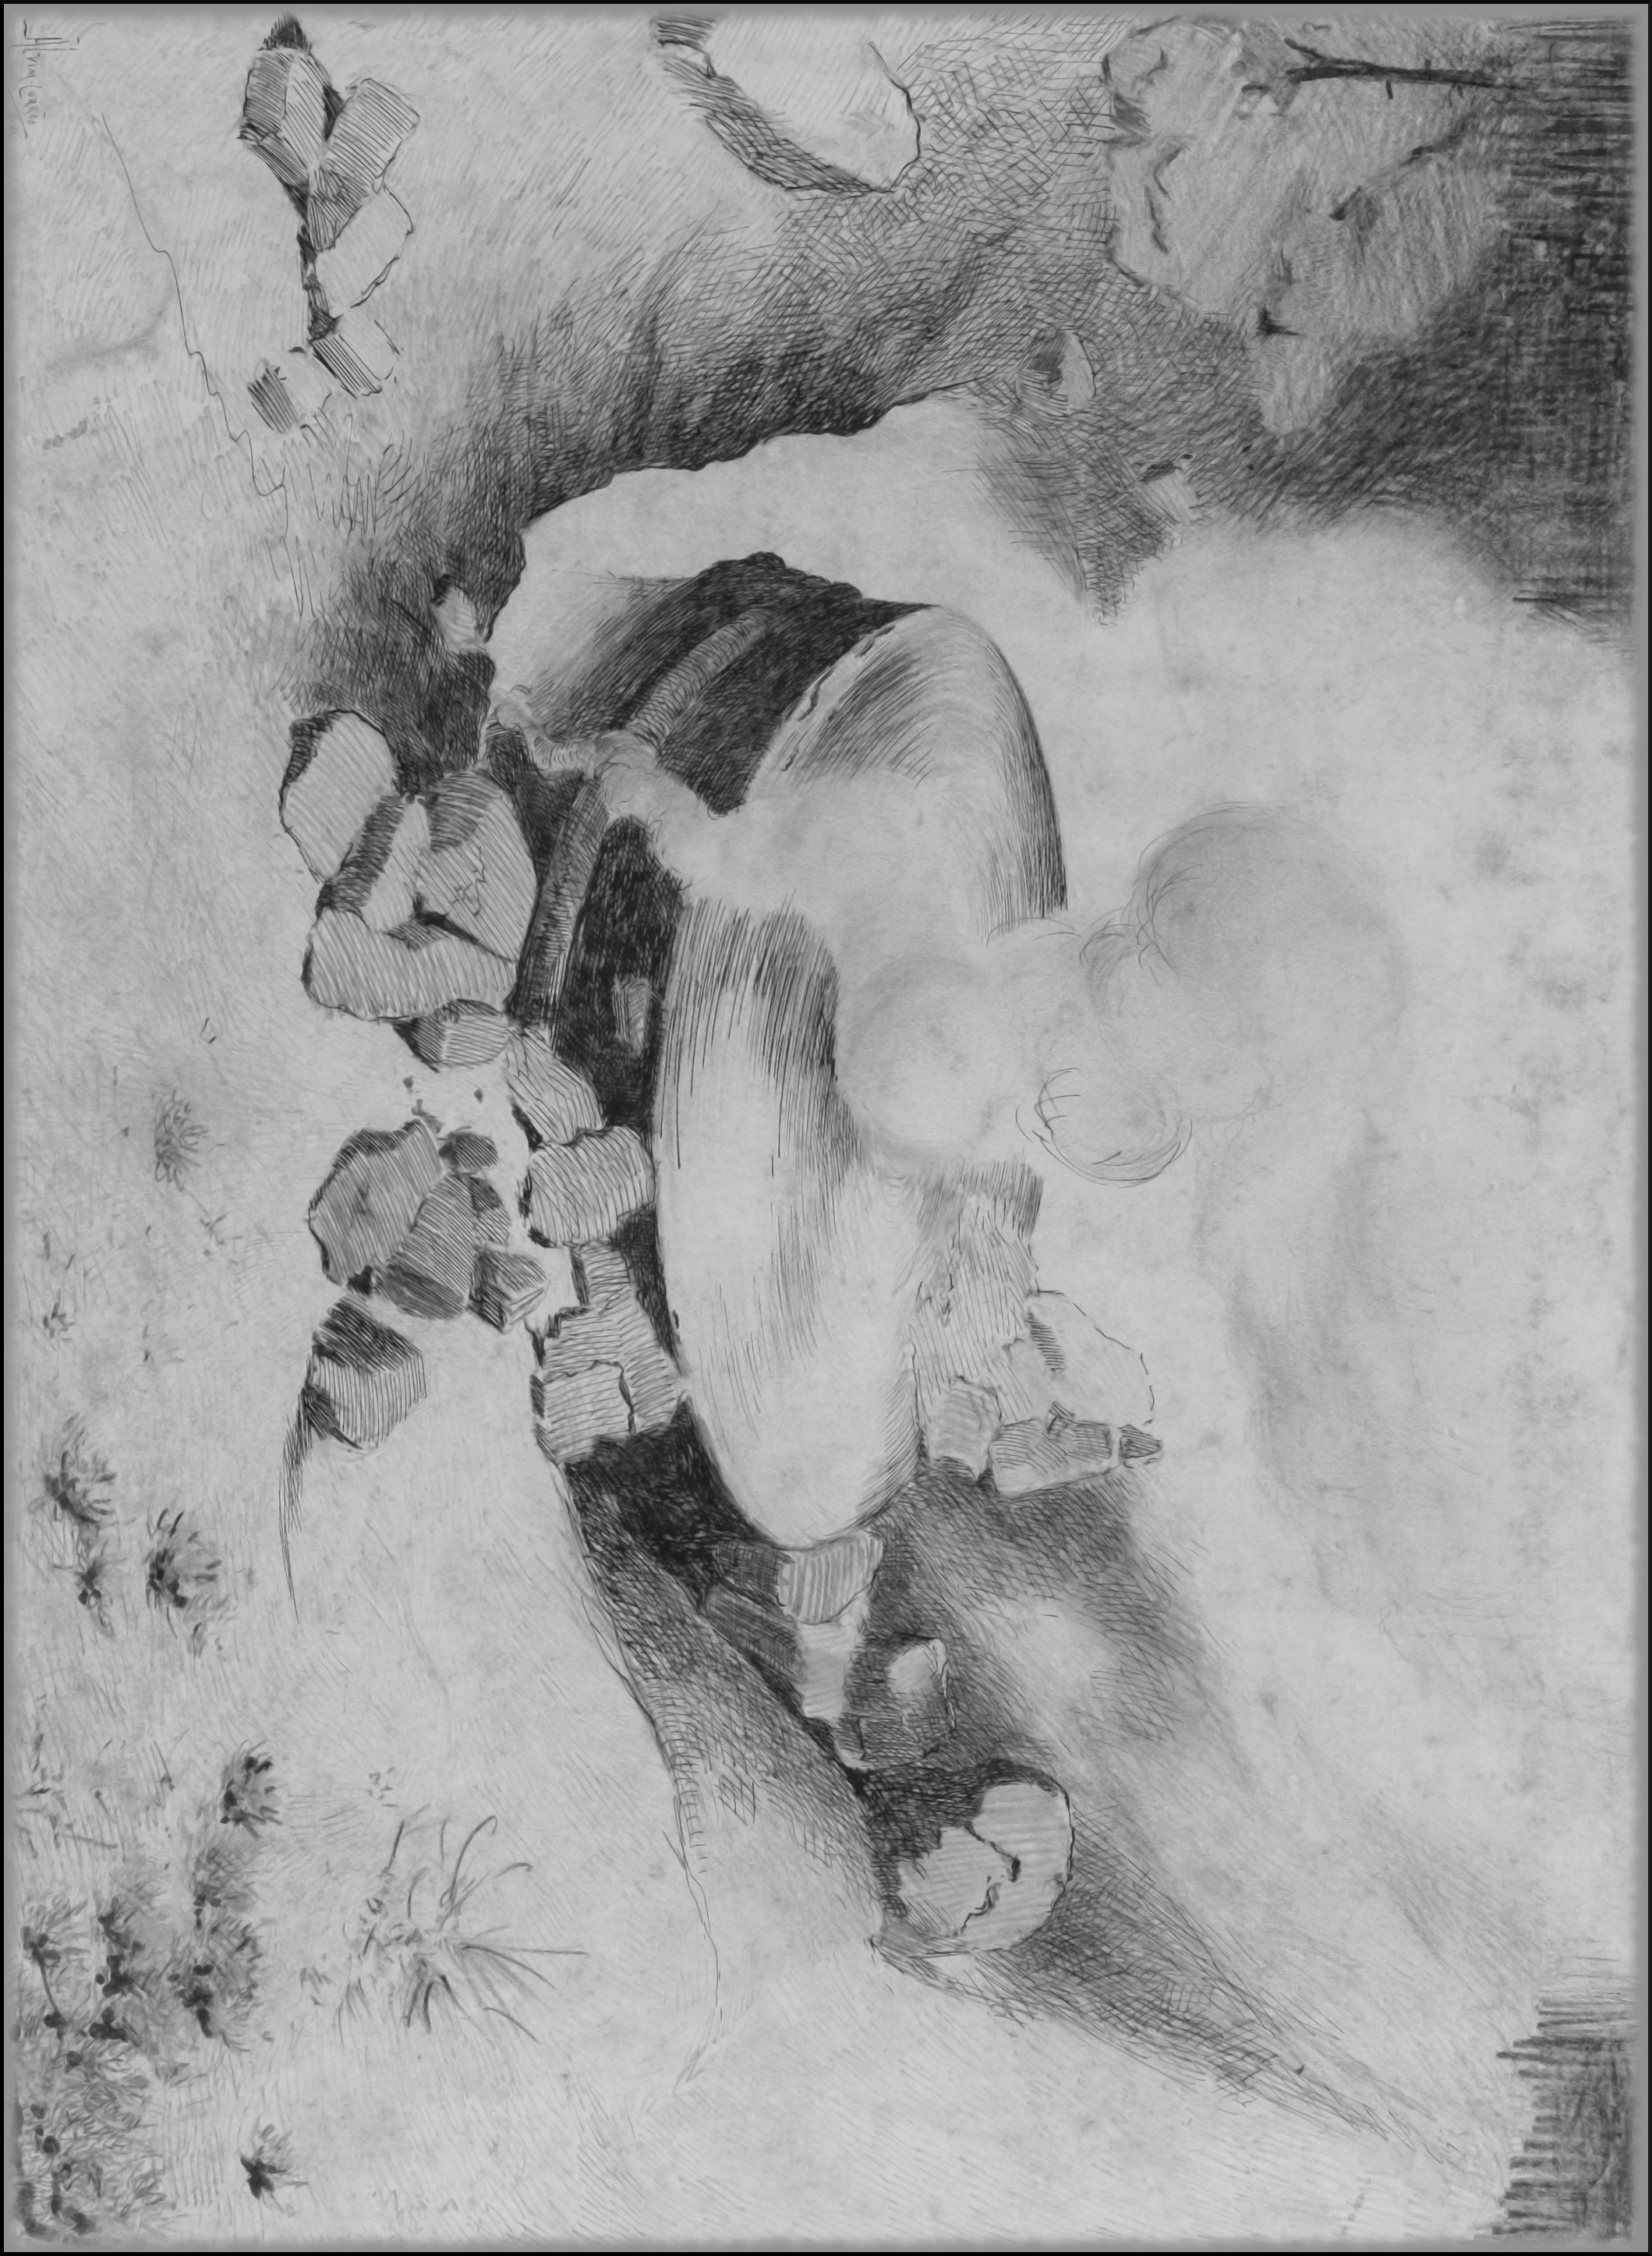
\includegraphics[width=.9\columnwidth]{3crater}
	\caption{It looked like a rusty gas float}
\end{sidewaysfigure}

At that time it was quite clear in my own mind that the Thing had come from the planet Mars, but I judged it improbable that it contained any living creature. I thought the unscrewing might be automatic. In spite of Ogilvy, I still believed that there were men in Mars. My mind ran fancifully on the possibilities of its containing manuscript, on the difficulties in translation that might arise, whether we should find coins and models in it, and so forth. Yet it was a little too large for assurance on this idea. I felt an impatience to see it opened. About eleven, as nothing seemed happening, I walked back, full of such thought, to my home in Maybury. But I found it difficult to get to work upon my abstract investigations.

In the afternoon the appearance of the common had altered very much. The early editions of the evening papers had startled London with enormous headlines:

\begin{center}\scshape
»A Message Received From Mars.«\\
»Remarkable Story From Woking,«
\end{center}

and so forth. In addition, Ogilvy's wire to the Astronomical Exchange had roused every observatory in the three kingdoms.

There were half a dozen flys or more from the Woking station standing in the road by the sand-pits, a basket-chaise from Chobham, and a rather lordly carriage. Besides that, there was quite a heap of bicycles. In addition, a large number of people must have walked, in spite of the heat of the day, from Woking and Chertsey, so that there was altogether quite a considerable crowd—one or two gaily dressed ladies among the others.

It was glaringly hot, not a cloud in the sky nor a breath of wind, and the only shadow was that of the few scattered pine trees. The burning heather had been extinguished, but the level ground towards Ottershaw was blackened as far as one could see, and still giving off vertical streamers of smoke. An enterprising sweet-stuff dealer in the Chobham Road had sent up his son with a barrow-load of green apples and ginger beer.

Going to the edge of the pit, I found it occupied by a group of about half a dozen men—Henderson, Ogilvy, and a tall, fair-haired man that I afterwards learned was Stent, the Astronomer Royal, with several workmen wielding spades and pickaxes. Stent was giving directions in a clear, high-pitched voice. He was standing on the cylinder, which was now evidently much cooler; his face was crimson and streaming with perspiration, and something seemed to have irritated him.


\begin{wrapfigure}{O}{0.6\textwidth}
\centering

\includegraphics[width=0.6\textwidth]{3tailpiece}
%\captionlistentry{Tailpiece to Chapter \thechapter}
\end{wrapfigure}




A large portion of the cylinder had been uncovered, though its lower end was still embedded. As soon as Ogilvy saw me among the staring crowd on the edge of the pit he called to me to come down, and asked me if I would mind going over to see Lord Hilton, the lord of the manor.

The growing crowd, he said, was becoming a serious impediment to their excavations, especially the boys. They wanted a light railing put up, and help to keep the people back. He told me that a faint stirring was occasionally still audible within the case, but that the workmen had failed to unscrew the top, as it afforded no grip to them. The case appeared to be enormously thick, and it was possible that the faint sounds we heard represented a noisy tumult in the interior.

I was very glad to do as he asked, and so become one of the privileged spectators within the contemplated enclosure. I failed to find Lord Hilton at his house, but I was told he was expected from London by the six o'clock train from Waterloo; and as it was then about a quarter past five, I went home, had some tea, and walked up to the station to waylay him.

